\documentclass{article}
\usepackage{graphicx} % Required for inserting images
\graphicspath{ {./Images/} }
\usepackage{pdfpages}
\newcommand{\insertslide}[2]{
\begin{center}
    \fbox{\includegraphics[page=#2,scale=0.25]{#1}}
\end{center}
}
% \insertslide{Slides/CM1.pdf}{1} to insert first page of CM1.pdf, for example.
\usepackage{amsmath}
\renewcommand{\familydefault}{\sfdefault}

\title{Notes LINFO1252}
\author{Quentin Bodart}
\date{Q1 2024-2025}

\begin{document}
\maketitle
\tableofcontents
\pagebreak

\section*{Objectifs du cours}
    \begin{itemize}
        \item utiliser et comprendre les systèmes informatiques (i.p. GNU/Linux)
        \item utiliser les services fournis par les SE (systèmes d'exploitation)
        \item design et mise en oeuvre d'un SE
    \end{itemize}

\section{CM 1}
    \subsection{Le système informatique et le rôle du système d’exploitation}
    \textbf{Syllabus} : https://sites.uclouvain.be/SystInfo/notes/Theorie/intro.html

        \subsubsection{Fondamentaux}
            \begin{itemize}
                \item Composants :
                \begin{itemize}
                    \item CPU / Processeur
                    \item Mémoire Principale (RAM)
                    \item Dispositifs d’entrée/sortie (y.c. de stockage)
                \end{itemize}
                \item Fonctionnement d'un CPU
                \begin{itemize}
                    \item Lire / écrire en mémoire vers / depuis des registres
                    \item Opérations (calculs, comparaisons) sur ces registres
                \end{itemize}
                \item Jeux d'instructions
                \begin{itemize}
                    \item x86\_64 (PC, anciens Mac)
                    \item ARM A64 (Raspberry PI, iPhone, nouveaux Mac M1–3)
                \end{itemize}
            \end{itemize}
        
        \subsubsection{Architecture de von Neumann}
            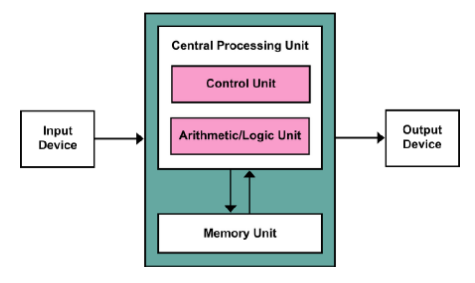
\includegraphics[scale = .5]{von_neumann.png}
        
        \subsubsection{Fonctionnement d'un système informatique}
            \begin{itemize}
                \item La représentation des données se fait en \textbf{binaire}.
                \item Les opérations d'entrée-sortie se déroule de manière concurrente.
                \item Il y existe des contrôleurs distinct controlant chacun un type de périphérique.
                \item Chaque contrôleur possède une mémoire dédiée (buffer)
                \item Le processeur doit déplacer des donnés depuis/vers la
                mémoire principale depuis/vers ces buffers dédiés
                \item Le processeur suit un "fil" continu d’instructions
                \item Le contrôleur de périphérique annonce au
                processeur la fin d’une opération d’entrée/sortie en
                générant une interruption (signal électrique à destination du processeur)
            \end{itemize}

        \subsubsection{Traitement d'une interruption}
            Le processeur interrompt le fil d’exécution d’instructions courant et
            transfert le contrôle du processeur à une routine de traitement.
            Cette même routine détermine la source de l'interruption, puis restaure l'état du processeur
            et reprend le processus :\\
            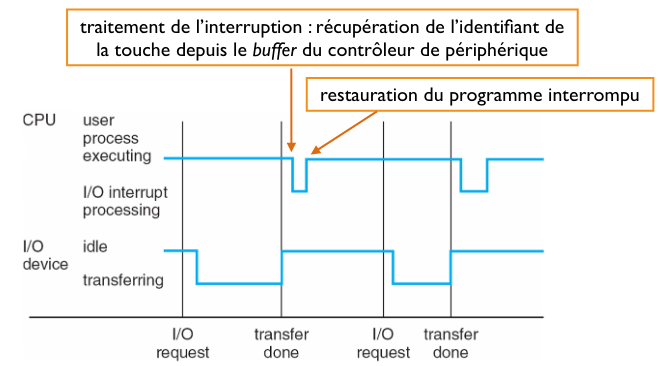
\includegraphics[scale=.75]{interruption.png}

        \subsubsection{Accès direct à la mémoire}
            Direct Memory Access (DMA) désigne le fait de ne pas faire une interruption à chaque octet lu depuis un disque dur.
            Une interruption est tout de même faite à la fin du transfert d'un \textbf{bloc}.
        
        \subsubsection{Système informatique complet}
            \includegraphics*[scale=.85]{systeme_complet.png}
        
        \subsubsection{Rôle du système d'exploitation}
            Programmer directement au-dessus du matériel, gérer les interruption, etc... serait une trop grosse tâche pour le programmeur.\\\\
            3 rôles principaux
            \begin{itemize}
                \item Rendre l’utilisation et le développement d’applications
                plus simple et plus universel (portable d’une machine à
                une autre)
                \item Permettre une utilisation plus efficace des ressources
                \item Assurer l’intégrité des données et des programmes
                entre eux (e.g., un programme crash mais pas le système)
            \end{itemize}
        
        \subsubsection{Virtualisation}
            Le système d'expoitation \textbf{virtualise} les ressources matérielles afin de fonctionner de la même manière sur des systèmes avec des ressources et composants fort différents.
            Chaque SE doit trouver un compromis entre abstraction et efficacité !

        \subsubsection{Séparation entre mécanisme et politique}
            \begin{itemize}
                \item Un mécanisme permet le partage de temps
                \item Une politique arbitre entre les processus pouvant s’exécuter
                et le(s) processeur(s) disponibles
            \end{itemize}
            On peut définir des politiques d’ordonnancement différentes selon les contextes, mais sur la base du même mécanisme.
        
        \subsubsection{Modes d'exécution}
            \begin{itemize}
                \item mode utilisateur : programme utilisant les abstractions
                fournies par le SE ; certaines instructions sont interdites, comme par exemple:
                \begin{itemize}
                    \item Accès à une zone mémoire non-autorisée (SegFault)
                    \item De manière générale, toutes les instructions permettant de
                    changer la configuration matérielle du système, comme la
                    configuration ou la désactivation des interruptions
                \end{itemize}
                \item mode protégé : utilisé par le noyau du SE, toutes les
                instructions sont autorisées
                \item L’utilisation de fonctionnalités du SE par un processus
                utilisateur nécessite de passer d’un mode à l’autre : \textbf{appel système}
            \end{itemize}
        
        \subsubsection{Appel système}
            \begin{itemize}
                \item Un appel système permet à un processus utilisateur
                d’invoquer une fonctionnalité du SE
                \item Le processeur interrompt le processus, passe en mode
                protégé, et branche vers le point d’entrée unique du noyau :\\
                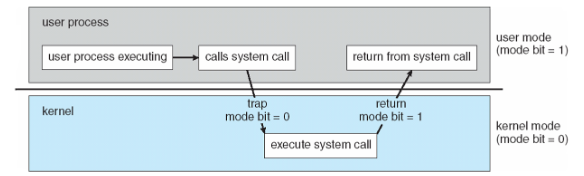
\includegraphics[scale=.75]{appel_systeme.png}
            \end{itemize}
                
            %TODO

    \subsection{Utilisation de la ligne de commande}
    \textbf{Syllabus} : https://sites.uclouvain.be/SystInfo/notes/
    Theorie/shell/shell.html

            \subsubsection{Utilitaires UNIX}
                La philosophie lors de la création des utilitaires UNIX était
                de créer des outils les plus simples possible,
                donc d'avoir une seule tâche par outil :\\
                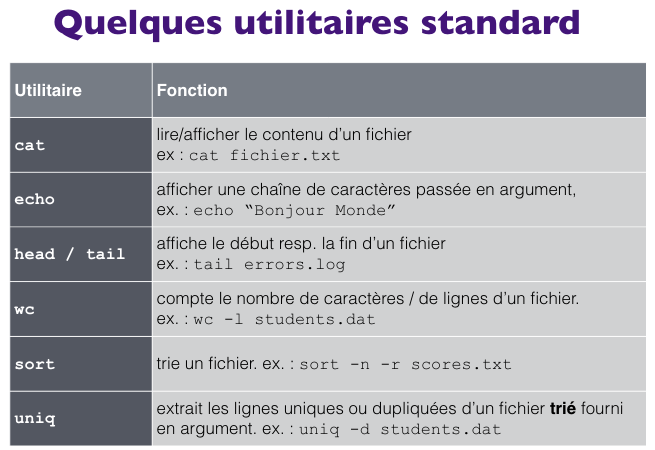
\includegraphics[scale=.5]{utilitaires_unix.png}
                Afin d'en savoir plus sur unecommande, il suffit d'utiliser l'utilitaire `man`.
            
            \subsubsection{Shell / Interpréteur de commandes}
                Rend possible l'interaction avec le SE.
                Il en existe plusieurs, mais le principal est `bash`.
                Il est toujours complémentaire à une \textbf{interface graphique}.
            
            \subsubsection{Flux et redirections}
                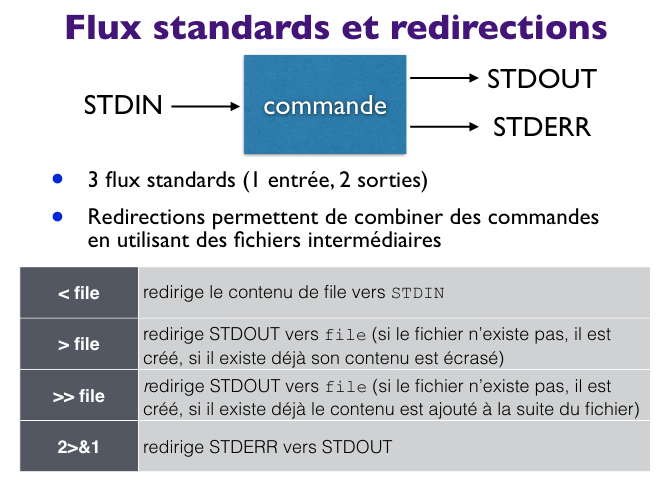
\includegraphics[scale=.5]{flux_std_et_redirections.png}\\
                Exemple de redirections :\\
                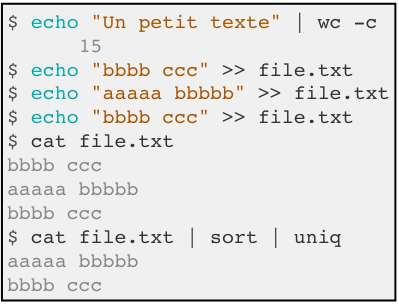
\includegraphics[scale=.5]{redirection_example.png}
            
                \subsubsection{Scripts}
                    Un système UNIX peut exécuter du language machine ou des \textbf{languages interprétés}
                    Un script commence par convention par les symboles $\#!$, référant à l'interpréteur, ici bin/bash :\\
                    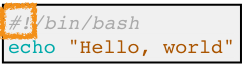
\includegraphics[scale=.7]{bash_script.png}\\\\
                    Ils peuvent aussi contenir des \textbf{variables}:\\
                    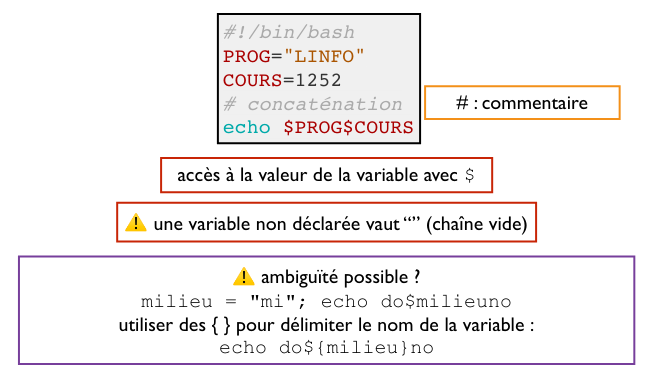
\includegraphics[scale=.5]{script_variables.png}\\\\
                    et des \textbf{conditionnelles} :\\
                    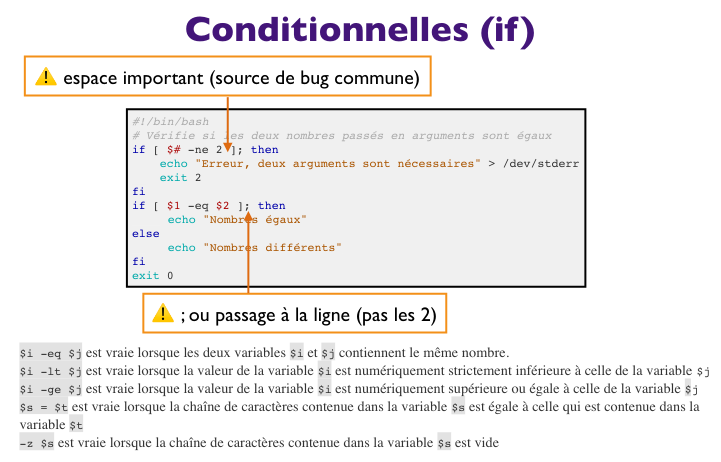
\includegraphics[scale=.4]{conditionnelles.png}\\
                    et des \textbf{boucles for}:\\
                    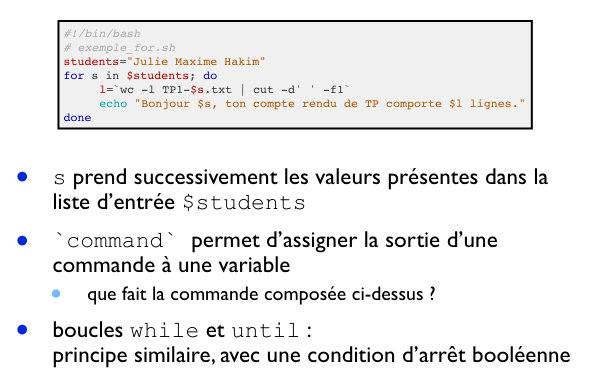
\includegraphics[scale=.6]{script_boucle_for.png}
\pagebreak
\section{CM2 : language C et compléments}
    \subsection{Le language C}
        Jusqu'en 1970, les OS étaient codés en assembleur, ce qui était 
        très chronophage et difficile à maintenir, d'où la nécessité d'un 
        language plus haut niveau, mais toujours proche de la machine : le C.
        Son objectif était de concevoir un language :
        \begin{itemize}
            \item Haut niveau (structuré)
            \item Proche du matériel (accès direct à la mémoire et traduction direct au processeur)
            \item Efficace (non-interprété et sans machine virtuelle)
            \item Portable
        \end{itemize}
        
        \subsubsection{Préprocesseur}
            Le code C est tout d’abord transformé par un
            préprocesseur avant d’être compilé en
            langage machine par le compilateur.\\
            Les directives telles que "\#include" ou "\#define" y sont remplacées
            par du texte spécifique à la commande.\\
            C'est seulement après ça que le code est compilé en code machine.

        \subsubsection{headers}
            Les directives \#include du préprocesseur permettent d’importer
            des définitions de fonctions, de constantes, etc. d’une librairie \\
            Séparation entre fichiers headers (.h) et sources (.c) :
            \begin{itemize}
                \item Le header contient la défnition des fonctions, suffisante pour savoir
                comment générer le code pour les appeler
                \item Le code source contient la mise en œuvre de ces fonctions
                \item \#include “monheader.h” pour inclure un header du dossier
                courant (du même projet)
                \item \#include $<$header.h$>$ pour inclure un header standard
            \end{itemize}
        
        \subsubsection{Intégration avec le shell}
            \insertslide{Slides/CM2.pdf}{15}
            Le tableau d'argument donné à main se termine toujours par NULL.
        
        \subsubsection{Affichage formatté}
            Pour afficher un String formatté en C, on peut utiliser la fonction printf:
            \insertslide{Slides/CM2.pdf}{16}
            Modificateurs (format specifiers):\\
            \begin{center}
                \begin{tabular}{|c|c|}
                    \hline
                    \%c & char \\
                    \hline
                    \%d / \%i & signed int \\
                    \hline
                    \%e / \%E & scientific notation \\
                    \hline
                    \%f & float \\
                    \hline
                    \%ld / \%li & long \\
                    \hline
                    \%lf & double \\
                    \hline
                    \%Lf & long double \\
                    \hline
                \end{tabular}
            \end{center}
    \subsection{Types de données}
        \begin{itemize}
            \item int, long : variable entière
            \item char : charactère
            \item double, float : nombre en virgule flottante
            \item booléens : définis dans stdbool.h, true ou false
            \item String : pas d'objet String en c, 
            seulement une chaîne de char $\rightarrow$ longueur de la chaîne inconnue !
            \item Structures de contrôle : while, for, if, ...
        \end{itemize}
        La taille occupée par un type de donnée peut être récupérée via \textbf{sizeof()}.
        \subsubsection{Nombres signés et flottants}
            Les entiers, en C, sont signés par défaut :
            \insertslide{Slides/CM2.pdf}{22}
            Via le mot-clé "unsigned", on peu "dé-signer" un type de donnée :
            \insertslide{Slides/CM2.pdf}{21}
            Représentation de nombres flottants:
            \insertslide{Slides/CM2.pdf}{23}
        
        \subsubsection{Caractères}
            Les caractères en C sont représentés par un nombre, en accord avec la
            norme ASCII.\\
            Deux types de charactères :
            \begin{itemize}
                \item 0x0....... : permet de représenter les caractères anglais
                \item 0x1....... : permet de représenter les caractères accentués
            \end{itemize}
            \insertslide{Slides/CM2.pdf}{26}
        
        \subsubsection{Chaînes de caractères}
            En C, une chaîne de charactères est stockée sous la forme d'un tableau.\\
            Le dernier élément du tableau contient le charactère "$\backslash$0".
\pagebreak
        \subsubsection{Pointeurs}
            Un \textbf{pointeur} est une variable qui contient l’adresse à
            laquelle est stockée un autre élément (variable, fonction, etc.)\\
            La mémoire peut être vue comme une suite de "cases" (octets) avec des 
            adresses consécutives (index de chaque octet).
            \begin{itemize}
                \item On peut créer un pointeur en utilisant le caractère "*" et récupérer
                une adresse en utilsant le caractère "\&".
                \item Le charctère "*" peut aussi être utilisée sur un pointeur pour récupérer sa valeur (déréférencement)
                \item En pratique, char[] et char* sont équivalents.
                \item Les pointeurs permettent de passer une variable par référence à une fonction.
            \end{itemize}
        
        \subsubsection{Pointeurs vers une fonction}
            Une fonction contient une séquence d'instructions, commençant à l'adresse
            où est stockée sa première instruction.\\
            On peut stocker l'adresse d'une fonction dans un \textbf{pointeur de fonction}:\\
            Déclaration : type (*ptr)([type\_arg]+)\\
            Exemple :
            \insertslide{Slides/CM2.pdf}{50}
        
        \subsubsection{Manipulation de bits}
            4 opérateurs binaires :
            \begin{itemize}
                \item tilde : inversion $\rightarrow$ tilde00000000 = 11111111
                \item \& : ET $\rightarrow$ 11111010 \& 01011111 = 01011010
                \item $|$ : OU $\rightarrow$ 11111010 $|$ 01011111 = 11111111
                \item \^ : OU exclusif $\rightarrow$ 11111010 \^ 01011111 = 10100101
            \end{itemize}
\pagebreak

\section{CM3 : Gestion de la mémoire}
    \subsection{Organisation d'un programme Linux en mémoire}
            Les différentes parties de la mémoire de Linux sont appelés \textbf{Segments}.\\
            Ceux qui nous intéressent:
            \begin{itemize}
                \item Segment 1 : \textbf{code}\\
                Il contient les instructions à exécuter par le processeur, directement extraites des codes.
                \item Segment 2 : \textbf{données initialisées}\\
                Contient les données initialisées par les codes du segment 1
                \item Segment 3 : \textbf{données non-initialisées}\\
                Contient les données non-initialisées par le codes du segment 1.\\
                Elles sont souvent initialisées à 0 par défaut, en attente d'être transférées dans le segment 2.
                \item Segment 4 : \textbf{Heap et Stack}
                \begin{itemize}
                    \item Heap : Permet aux programmes d'y réserver des zones mémoire\\(c.f. malloc, free, valgrind)
                    \item Stack : Permet de stocker les variables locales et les appels de fonctions, ainsi que de récupérer les valeurs de retour.
                \end{itemize}
                \item Segment 5 : \textbf{Arguments et variables d'environnement}
            \end{itemize}
        \insertslide{Slides/CM3}{6}
\pagebreak
    \subsection{Gestion de la mémoire dynamique}
        malloc() et free() ne sont pas mises en oeuvre dans le noyau du système d'exploitation, ce sont simplement des \textbf{fonctions da la librairie standard utilisant des appels système : brk() et sbrk()}.\\\\
        malloc() est aligné sur un \textbf{facteur d'alignement} : elle retourne un nombre entier d'octets directement supérieur au nombre d'octets demandés. (padding)\\
        Exemple : Sous Linux, ce facteur est de \textbf{16 octets}. Si l'on demande 37 octets, le malloc va en retourner 64.
        \subsubsection{Objectif d'un algorithme de gestion de mémoire dynamique}
            Les objectifs de cet algorithme sont les suivants :
            \begin{itemize}
                \item \textbf{Minimiser le temps d'exécution} et maximiser sa stabilité
                \item \textbf{Utiliser efficacement la mémoire} (minimiser la fragmentation):\\
                Deux types de fragmentation:
                \begin{itemize}
                    \item Fragmentation interne : espace perdu par le padding
                    \item Fragmentation externe : espace perdu par l'allocation et désallocation de la mémoire
                \end{itemize}
                \item \textbf{Bonnes propriétés de localité spatiale} :\\
                Alloue les variables proches les unes des autres afin d'accélérer l'accès du cache du processeur
            \end{itemize}
        
        \subsubsection{Implémentation de l'algorithme}
            Une des implémentations pourrait utiliser des métadonnées :
            \insertslide{Slides/CM3}{48}
\pagebreak
            Cependant, aucune des implémentations ne peut satisfaire les 3 conditions parfaitement.
            Par exemple :
            \insertslide{Slides/CM3}{55}
\pagebreak
\section{CM4 : Structure des ordinateurs}
    \subsection{Organisation d'un système informatique}
        \begin{itemize}
            \item La mémoire est adressée par \textbf{bytes}.
            \item Les adresses sont généralement écrites sur 32 ou 64 bits. (64 bits permettent environ 1,8e19 valeurs différentes)
            \item Les instructions sont aussi codées en binaire, elles aussi de taille variable
        \end{itemize}

        \subsubsection{Mémoire du processeur}
            Il en existe deux types :
            \begin{itemize}
                \item SRAM : généralement très chère et rapide, présente dans les processeurs modernes (cache)
                \item DRAM : beaucoup moins chère, mais bien plus grande capacité et modulaire
            \end{itemize}
Redondant, il est chiant ce cours...
\end{document}